\documentclass[]{article}
\usepackage{lmodern}
\usepackage{amssymb,amsmath}
\usepackage{ifxetex,ifluatex}
\usepackage{fixltx2e} % provides \textsubscript
\ifnum 0\ifxetex 1\fi\ifluatex 1\fi=0 % if pdftex
  \usepackage[T1]{fontenc}
  \usepackage[utf8]{inputenc}
\else % if luatex or xelatex
  \ifxetex
    \usepackage{mathspec}
  \else
    \usepackage{fontspec}
  \fi
  \defaultfontfeatures{Ligatures=TeX,Scale=MatchLowercase}
\fi
% use upquote if available, for straight quotes in verbatim environments
\IfFileExists{upquote.sty}{\usepackage{upquote}}{}
% use microtype if available
\IfFileExists{microtype.sty}{%
\usepackage{microtype}
\UseMicrotypeSet[protrusion]{basicmath} % disable protrusion for tt fonts
}{}
\usepackage[margin=1in]{geometry}
\usepackage{hyperref}
\hypersetup{unicode=true,
            pdftitle={hw3},
            pdfauthor={Pablo, Román, Sofia},
            pdfborder={0 0 0},
            breaklinks=true}
\urlstyle{same}  % don't use monospace font for urls
\usepackage{color}
\usepackage{fancyvrb}
\newcommand{\VerbBar}{|}
\newcommand{\VERB}{\Verb[commandchars=\\\{\}]}
\DefineVerbatimEnvironment{Highlighting}{Verbatim}{commandchars=\\\{\}}
% Add ',fontsize=\small' for more characters per line
\usepackage{framed}
\definecolor{shadecolor}{RGB}{248,248,248}
\newenvironment{Shaded}{\begin{snugshade}}{\end{snugshade}}
\newcommand{\AlertTok}[1]{\textcolor[rgb]{0.94,0.16,0.16}{#1}}
\newcommand{\AnnotationTok}[1]{\textcolor[rgb]{0.56,0.35,0.01}{\textbf{\textit{#1}}}}
\newcommand{\AttributeTok}[1]{\textcolor[rgb]{0.77,0.63,0.00}{#1}}
\newcommand{\BaseNTok}[1]{\textcolor[rgb]{0.00,0.00,0.81}{#1}}
\newcommand{\BuiltInTok}[1]{#1}
\newcommand{\CharTok}[1]{\textcolor[rgb]{0.31,0.60,0.02}{#1}}
\newcommand{\CommentTok}[1]{\textcolor[rgb]{0.56,0.35,0.01}{\textit{#1}}}
\newcommand{\CommentVarTok}[1]{\textcolor[rgb]{0.56,0.35,0.01}{\textbf{\textit{#1}}}}
\newcommand{\ConstantTok}[1]{\textcolor[rgb]{0.00,0.00,0.00}{#1}}
\newcommand{\ControlFlowTok}[1]{\textcolor[rgb]{0.13,0.29,0.53}{\textbf{#1}}}
\newcommand{\DataTypeTok}[1]{\textcolor[rgb]{0.13,0.29,0.53}{#1}}
\newcommand{\DecValTok}[1]{\textcolor[rgb]{0.00,0.00,0.81}{#1}}
\newcommand{\DocumentationTok}[1]{\textcolor[rgb]{0.56,0.35,0.01}{\textbf{\textit{#1}}}}
\newcommand{\ErrorTok}[1]{\textcolor[rgb]{0.64,0.00,0.00}{\textbf{#1}}}
\newcommand{\ExtensionTok}[1]{#1}
\newcommand{\FloatTok}[1]{\textcolor[rgb]{0.00,0.00,0.81}{#1}}
\newcommand{\FunctionTok}[1]{\textcolor[rgb]{0.00,0.00,0.00}{#1}}
\newcommand{\ImportTok}[1]{#1}
\newcommand{\InformationTok}[1]{\textcolor[rgb]{0.56,0.35,0.01}{\textbf{\textit{#1}}}}
\newcommand{\KeywordTok}[1]{\textcolor[rgb]{0.13,0.29,0.53}{\textbf{#1}}}
\newcommand{\NormalTok}[1]{#1}
\newcommand{\OperatorTok}[1]{\textcolor[rgb]{0.81,0.36,0.00}{\textbf{#1}}}
\newcommand{\OtherTok}[1]{\textcolor[rgb]{0.56,0.35,0.01}{#1}}
\newcommand{\PreprocessorTok}[1]{\textcolor[rgb]{0.56,0.35,0.01}{\textit{#1}}}
\newcommand{\RegionMarkerTok}[1]{#1}
\newcommand{\SpecialCharTok}[1]{\textcolor[rgb]{0.00,0.00,0.00}{#1}}
\newcommand{\SpecialStringTok}[1]{\textcolor[rgb]{0.31,0.60,0.02}{#1}}
\newcommand{\StringTok}[1]{\textcolor[rgb]{0.31,0.60,0.02}{#1}}
\newcommand{\VariableTok}[1]{\textcolor[rgb]{0.00,0.00,0.00}{#1}}
\newcommand{\VerbatimStringTok}[1]{\textcolor[rgb]{0.31,0.60,0.02}{#1}}
\newcommand{\WarningTok}[1]{\textcolor[rgb]{0.56,0.35,0.01}{\textbf{\textit{#1}}}}
\usepackage{longtable,booktabs}
\usepackage{graphicx,grffile}
\makeatletter
\def\maxwidth{\ifdim\Gin@nat@width>\linewidth\linewidth\else\Gin@nat@width\fi}
\def\maxheight{\ifdim\Gin@nat@height>\textheight\textheight\else\Gin@nat@height\fi}
\makeatother
% Scale images if necessary, so that they will not overflow the page
% margins by default, and it is still possible to overwrite the defaults
% using explicit options in \includegraphics[width, height, ...]{}
\setkeys{Gin}{width=\maxwidth,height=\maxheight,keepaspectratio}
\IfFileExists{parskip.sty}{%
\usepackage{parskip}
}{% else
\setlength{\parindent}{0pt}
\setlength{\parskip}{6pt plus 2pt minus 1pt}
}
\setlength{\emergencystretch}{3em}  % prevent overfull lines
\providecommand{\tightlist}{%
  \setlength{\itemsep}{0pt}\setlength{\parskip}{0pt}}
\setcounter{secnumdepth}{0}
% Redefines (sub)paragraphs to behave more like sections
\ifx\paragraph\undefined\else
\let\oldparagraph\paragraph
\renewcommand{\paragraph}[1]{\oldparagraph{#1}\mbox{}}
\fi
\ifx\subparagraph\undefined\else
\let\oldsubparagraph\subparagraph
\renewcommand{\subparagraph}[1]{\oldsubparagraph{#1}\mbox{}}
\fi

%%% Use protect on footnotes to avoid problems with footnotes in titles
\let\rmarkdownfootnote\footnote%
\def\footnote{\protect\rmarkdownfootnote}

%%% Change title format to be more compact
\usepackage{titling}

% Create subtitle command for use in maketitle
\providecommand{\subtitle}[1]{
  \posttitle{
    \begin{center}\large#1\end{center}
    }
}

\setlength{\droptitle}{-2em}

  \title{hw3}
    \pretitle{\vspace{\droptitle}\centering\huge}
  \posttitle{\par}
    \author{Pablo, Román, Sofia}
    \preauthor{\centering\large\emph}
  \postauthor{\par}
      \predate{\centering\large\emph}
  \postdate{\par}
    \date{25/2/2020}


\begin{document}
\maketitle

\begin{verbatim}
## 
## Attaching package: 'dplyr'
\end{verbatim}

\begin{verbatim}
## The following objects are masked from 'package:stats':
## 
##     filter, lag
\end{verbatim}

\begin{verbatim}
## The following objects are masked from 'package:base':
## 
##     intersect, setdiff, setequal, union
\end{verbatim}

\begin{verbatim}
## Warning: package 'factoextra' was built under R version 3.6.3
\end{verbatim}

\begin{verbatim}
## Welcome! Want to learn more? See two factoextra-related books at https://goo.gl/ve3WBa
\end{verbatim}

\begin{verbatim}
## Warning: package 'devtools' was built under R version 3.6.3
\end{verbatim}

\begin{verbatim}
## Loading required package: usethis
\end{verbatim}

\begin{verbatim}
## Warning: package 'usethis' was built under R version 3.6.3
\end{verbatim}

\begin{verbatim}
## Warning: package 'gridExtra' was built under R version 3.6.3
\end{verbatim}

\begin{verbatim}
## 
## Attaching package: 'gridExtra'
\end{verbatim}

\begin{verbatim}
## The following object is masked from 'package:dplyr':
## 
##     combine
\end{verbatim}

\#\#Ejercicio 1

\begin{Shaded}
\begin{Highlighting}[]
\KeywordTok{library}\NormalTok{(}\StringTok{'png'}\NormalTok{)}
\end{Highlighting}
\end{Shaded}

\#\#Ejercicio 2 Con los datos del archivo T8-4.DAT que corresponden a
tasas de rendimiento de cinco acciones listadas en NYSE:

\#\#\#\#\#a) Obtener la matriz muestral de covarianzas S y obtener las
componentes principales.

Para eso scamos la matriz de covarianzas \(S\) que es la siguiente.

\begin{verbatim}
##              V1           V2           V3           V4           V5
## V1 0.0016299269 0.0008166676 0.0008100713 0.0004422405 0.0005139715
## V2 0.0008166676 0.0012293759 0.0008276330 0.0003868550 0.0003109431
## V3 0.0008100713 0.0008276330 0.0015560763 0.0004872816 0.0004624767
## V4 0.0004422405 0.0003868550 0.0004872816 0.0008023323 0.0004084734
## V5 0.0005139715 0.0003109431 0.0004624767 0.0004084734 0.0007587370
\end{verbatim}

Ahora para calcular las componentes principales encontraremos sus
egienvecores.

\begin{verbatim}
##      [,1]  [,2]  [,3]  [,4]  [,5]
## [1,] 0.56 -0.74  0.13 -0.28  0.21
## [2,] 0.47  0.09  0.47  0.69 -0.28
## [3,] 0.55  0.65  0.11 -0.50  0.10
## [4,] 0.29  0.11 -0.61  0.44  0.58
## [5,] 0.28 -0.07 -0.62 -0.06 -0.73
\end{verbatim}

De donde obtenemos los componentes principales. \[\begin{array}{l}
Y_{1} = e_{1}^TX = 0.56X_{1} + 0.47X_{2}+ 0.55X_{3} + 0.29X_{4} + 0.28X_{5}\\
Y_{2} = e_{2}^TX = -0.74X_{1} + 0.09X_{2} + 0.65X_{3} + 0.11X_{4} - 0.07X_{5}\\
Y_{3} = e_{3}^TX = 0.13X_{1} + 0.47X_{2} +0.11X_{3} - 0.61X_{4} - 0.62X_{5}\\
Y_{4} = e_{4}^TX = -0.28X_{1} + 0.69X_{2} - 0.50X_{3} + 0.44X_{4} - 0.06X_{5}\\
Y_{5} = e_{5}^TX = 0.21X_{1} - 0.28X_{2} + 0.10X_{3} +  0.58X_{4} - 0.73X_{5}\\
\end{array}\]

\#\#\#\#\#b) Hacer la gráfica de codo correspondiente, y decidir cuáles
son las componentes más significativas. Realizar una propuesta de
interpretación para las dos primeras componentes.

Para realizar esto, veremos que tanta varianza aporta cada componente
principal, mediante el siguiente razonamiento.

\[\frac{\lambda_{k}}{\lambda_{1} + ... + \lambda_{k}}\]

\begin{verbatim}
## [1] 0.60159252 0.13255027 0.12322412 0.08511218 0.05752091
\end{verbatim}

\includegraphics{hw3_files/figure-latex/unnamed-chunk-6-1.pdf}

Podemos ver que la primer componente exlica un \(60\%\) mientras que las
componentes \(Y_{2},Y_{3},Y_{4},\) explican casi un \(10\%\) y la ultima
componente unicamente \(5\%\). La componente mas significativa es la
primera.

Una interpretacion para la primer componente principal seria una especie
de promedio ponderado pues todas las variables estan multiplicadas por
un coeficiente que les da peso con respecto a que tanta varianza
aportan. Mientras que la segunda componente principal podria ser una
donde se contrasta la primera columna y la ultima contra el resto.

\#\#\#\#\#c) Construir los intervalos simultáneos bonferronizados de
90\% para las varianzas λ1, λ2, λ3 de las primeras tres componentes Y1,
Y2, Y3.

Para obtener los intervalos de confianza simultaneos de Bonferroni al
\(100(1-\alpha)\%\) de confianza para \(\lambda_{i}\) se construiran de
la siguiente manera.

\[\frac{\hat{\lambda_{i}}}{1 + z(\frac{\alpha}{2m})\sqrt{\frac{2}{n}}}\le \lambda_{i} \le \frac{\hat{\lambda_{i}}}{1 - z(\frac{\alpha}{2m})\sqrt{\frac{2}{n}}} \]

\begin{verbatim}
## [1] 0.003135766 0.004212885
\end{verbatim}

\begin{verbatim}
## [1] 0.0006909105 0.0009282347
\end{verbatim}

\begin{verbatim}
## [1] 0.0006422984 0.0008629247
\end{verbatim}

\#\#\#\#\#d)¿Se puede resumir la variabilidad de los datos en menos de 5
dimensiones? Explicar.

Si podriamos ya que con las primeras tres componentes principales
\(Y_{1},Y_{2},Y_{3}\) acumulamos un total del \(80\%\) de viarianza
acumulada, con lo cual podria representarse suficientemente bien el
resto de los datos.

\#\#\#\#\#e) Replicar este ejercicio, pero tomando datos de 5 acciones
de la Bolsa Mexicana de Valores, con los datos que puedan conseguir del
año 2017.

Para eso Sacamos los rendimientos diarios de TV Azteca (AZTECACPO),
Televisa (TELEVISACPO),Wal Mart Mexico (WALMEX), Chedrahui (CHDRAUIB) y
Soriana (SORIANAB)

\begin{verbatim}
##   AZTECACPO TELEVISACPO WALMEX CHDRAUIB SORIANAB
## 1     -0.90      191.15  11.73     8.20     7.03
## 2      0.56       -0.31   0.87     1.72     0.80
## 3      7.05        0.16   0.71    -0.10     1.12
## 4     -0.90       -0.28   0.49     0.13    -0.76
## 5      0.42       -0.17  -0.34     0.09    -0.64
## 6     -0.31        0.74  -0.22     0.29     1.08
\end{verbatim}

Sacamos su matriz de covarianza \(S\) que es la siguiente.

\begin{verbatim}
##               AZTECACPO TELEVISACPO     WALMEX   CHDRAUIB   SORIANAB
## AZTECACPO   136.9573070   -1.340495  0.2784707 -1.0723353   2.288135
## TELEVISACPO  -1.3404951  148.539476 10.1932520  6.2090367   2.677804
## WALMEX        0.2784707   10.193252  2.2899164  0.6419263   1.048935
## CHDRAUIB     -1.0723353    6.209037  0.6419263  3.1537755   4.676990
## SORIANAB      2.2881349    2.677804  1.0489352  4.6769902 289.843582
\end{verbatim}

Sacamos sus componentes principales.

\begin{verbatim}
##      [,1]  [,2]  [,3]  [,4]  [,5]
## [1,] 0.01 -0.11  0.99  0.01  0.00
## [2,] 0.02  0.99  0.11 -0.05 -0.06
## [3,] 0.00  0.07  0.01  0.15  0.99
## [4,] 0.02  0.04  0.00  0.99 -0.16
## [5,] 1.00 -0.02 -0.02 -0.02  0.00
\end{verbatim}

De donde obtenemos los siguientes. \[\begin{array}{l}
Y_{1} = e_{1}^TX =  0.01X_{1} + 0.02X_{2} + 0.02X_{4} + X_{5}\\
Y_{2} = e_{2}^TX = -0.11X_{1} + 0.99X_{2} + 0.07X_{3} + 0.04X_{4} - 0.02X_{5}\\
Y_{3} = e_{3}^TX =  0.99X_{1} + 0.11X_{2} + 0.01X_{3} - 0.02X_{5}\\
Y_{4} = e_{4}^TX = -0.01X_{1} - 0.19X_{2} + 0.15X_{3} + 0.99X_{4} - 0.02X_{5}\\
Y_{5} = e_{5}^TX = - 0.06X_{2} + 0.99X_{3} + 0.16X_{4}\\
\end{array}\]

La grafica de codo es la siguiente.

\begin{Shaded}
\begin{Highlighting}[]
\NormalTok{lsum2 <-}\StringTok{ }\KeywordTok{sum}\NormalTok{(eig2}\FloatTok{.2}\OperatorTok{$}\NormalTok{values)}

\NormalTok{(var2}\FloatTok{.2}\NormalTok{ <-}\StringTok{  }\KeywordTok{aport_var}\NormalTok{(eig2}\FloatTok{.2}\OperatorTok{$}\NormalTok{values,lsum2))}
\end{Highlighting}
\end{Shaded}

\begin{verbatim}
## [1] 0.499347270 0.257595881 0.235503948 0.004888115 0.002664786
\end{verbatim}

\begin{Shaded}
\begin{Highlighting}[]
\KeywordTok{plot}\NormalTok{(var2}\FloatTok{.2}\NormalTok{,}\DataTypeTok{type=}\StringTok{"o"}\NormalTok{,}\DataTypeTok{ylab =} \StringTok{"Porcentaje de varianza expresada"}\NormalTok{, }\DataTypeTok{xlab =} \StringTok{"Componente"}\NormalTok{)}
\end{Highlighting}
\end{Shaded}

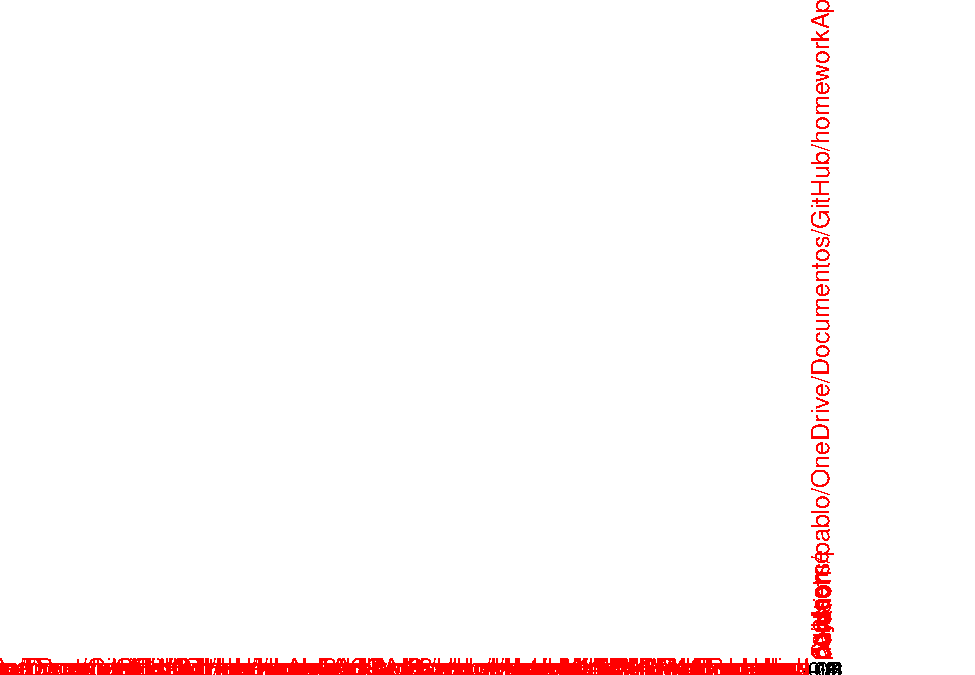
\includegraphics{hw3_files/figure-latex/unnamed-chunk-11-1.pdf}

Podemos ver que la primer componente exlica un \(50\%\) mientras que las
componentes \(Y_{2},Y_{3}\) explican casi un \(25\%\) y la ultimas
componentes \(Y_{4},Y_{5}\) practicamente no explican nada. La
componente pas significativa es la primera.

La interpretación es que son variables bastante ajenas aunque hubieramos
pensado que habria alguna relación entre las acciones de las televisoras
y las acciones de los supermercados. La primer componente \(Y_{1}\) le
otorga todo el peso a la variable \emph{Soriana} mientras que la segunda
\(Y_{2}\) muestra una relacion inversa entre las televisoras dandole
mayo peso a \emph{Televisa}. La tercera \(Y_3\) practicamente es la
inversa de \(Y_{2}\) da todo el peso a \emph{TV Azteca} y un peso igual
de pequeño a \emph{Televisa} de esta podriamos deducir si no lo
supieramos que estan en competencia y son bienes sustitutos. Para
\(Y_4\) le da practicamente todo el peso a \emph{Soriana}, y pesos casi
cero al resto.\(Y_5\) es la unica que agrupa de manera positiva a
\emph{Walmart} con \emph{Soriana} dandole casi todo el peso a
\emph{Walmart}, como esta casi no aporta varinza al modelo podriamos
interpretar que es una variable algo ajena en los datos. Lo cual hace
sentido.

Acontinuación mostraremos los intervalos simultaneos de bonferroni para
\(\lambda_i\) con \(i = 1,2,3\).

\begin{verbatim}
## [1] 2.654091e+02 3.962738e-03
\end{verbatim}

\begin{verbatim}
## [1] 1.369153e+02 8.731192e-04
\end{verbatim}

\begin{verbatim}
## [1] 1.251732e+02 8.116871e-04
\end{verbatim}

Podemos concluir este ejercicio diciendo que no bastaria con las
primeras dos componentes principales para explicar la variabilidad de
los datos, sino con las primeras tres componentes principales
\(Y_{1},Y_{2},Y_{3}\) acumulamos un total de casi \(99\%\) de viarianza
acumulada.

\hypertarget{ejercicio-3}{%
\subsection{Ejercicio 3}\label{ejercicio-3}}

\hypertarget{a.-comparar-estimaciones}{%
\subparagraph{3a. Comparar
estimaciones}\label{a.-comparar-estimaciones}}

Veamos:

\begin{itemize}
\item
  El \emph{error relativo para los scores} de las CP's, calculado por la
  \(|| . ||_{\infty}\) es: 2.8311423
\item
  El vector con los errores relativos para \(\lambda\)'s estimadas es

  \begin{longtable}[]{@{}lc@{}}
  \toprule
  & lambda\tabularnewline
  \midrule
  \endhead
  Comp.1 & -1.7117792\tabularnewline
  Comp.2 & -0.9300589\tabularnewline
  Comp.3 & -0.9090022\tabularnewline
  Comp.4 & -0.0005601\tabularnewline
  Comp.5 & -0.0002891\tabularnewline
  \bottomrule
  \end{longtable}
\end{itemize}

Se puede concluir que el cambio de escala SÍ afecta la estimación de los
componentes principales, y por mucho.

\hypertarget{b.-interpretacion}{%
\subparagraph{3b. Interpretación}\label{b.-interpretacion}}

\includegraphics{hw3_files/figure-latex/cpa analisis-1.pdf}
\includegraphics{hw3_files/figure-latex/cpa analisis-2.pdf}

\begin{verbatim}
## 
## Loadings:
##    Comp.1 Comp.2 Comp.3 Comp.4 Comp.5
## V1  0.781                0.542  0.302
## V2  0.306  0.764 -0.162 -0.545       
## V3  0.334                      -0.937
## V4  0.426 -0.579  0.220 -0.636  0.172
## V5         0.262  0.962              
## 
##                Comp.1 Comp.2 Comp.3 Comp.4 Comp.5
## SS loadings       1.0    1.0    1.0    1.0    1.0
## Proportion Var    0.2    0.2    0.2    0.2    0.2
## Cumulative Var    0.2    0.4    0.6    0.8    1.0
\end{verbatim}

\begin{verbatim}
## 
## Loadings:
##    Comp.1 Comp.2 Comp.3 Comp.4 Comp.5
## V1         0.782         0.541  0.302
## V2         0.350  0.764 -0.540       
## V3         0.327 -0.101        -0.938
## V4         0.391 -0.632 -0.642  0.172
## V5 -0.994                            
## 
##                Comp.1 Comp.2 Comp.3 Comp.4 Comp.5
## SS loadings       1.0    1.0    1.0    1.0    1.0
## Proportion Var    0.2    0.2    0.2    0.2    0.2
## Cumulative Var    0.2    0.4    0.6    0.8    1.0
\end{verbatim}

Para el caso de los datos originales, \(Y_{1}\) es una ponderación de
las 5 variables, dándole mayor peso a la primer variable. La segunda CP
es una distinción entre la segunda variable y quinta variable contra la
cuarta.

En el caso de los datos modificados, \(Y_{1}^{'}\) se inclina
\emph{totalmente} hacia la última variable. Mientras que la segunda
componente es un ponderaje de las primeras cuatro variables originales,
se observa con mayor claridad en el \emph{biplot}.

\hypertarget{c.-describir-efectos}{%
\subparagraph{3c. Describir efectos}\label{c.-describir-efectos}}

Vemos que el cambio de escala distorciona por completo los componentes
principales y por ende su interpretación. Es recomendable en este caso
usar \(R\), o lo que es lo mismo, \emph{estandarizar} los datos
(studentizarlos).

\#\#Ejercicio 4 Cargamos los datos y elegimos los que queremos analizar.

\begin{Shaded}
\begin{Highlighting}[]
\NormalTok{DATA<-}\KeywordTok{read.table}\NormalTok{(}\StringTok{"T110.DAT"}\NormalTok{, }\DataTypeTok{header=}\NormalTok{F)}
\NormalTok{X<-DATA[,}\OperatorTok{-}\KeywordTok{c}\NormalTok{(}\DecValTok{1}\NormalTok{,}\DecValTok{2}\NormalTok{)]}
\end{Highlighting}
\end{Shaded}

Estandarizamos los datos porque sus unidades son distintas

\begin{Shaded}
\begin{Highlighting}[]
\NormalTok{X_std <-}\StringTok{ }\KeywordTok{scale}\NormalTok{(X)}
\end{Highlighting}
\end{Shaded}

Obtenemos la matriz de covarianzas

\begin{Shaded}
\begin{Highlighting}[]
\NormalTok{cov<-}\KeywordTok{cov}\NormalTok{(X_std)}
\end{Highlighting}
\end{Shaded}

Encontramos sus eigenvalores y eigenvectores. Un vector propio es una
dirección y un valor propio es un número que indica cuánta varianza hay
en los datos en esa dirección.

\begin{Shaded}
\begin{Highlighting}[]
\NormalTok{ei<-}\KeywordTok{eigen}\NormalTok{(cov)}
\end{Highlighting}
\end{Shaded}

El valor propio más grande es el primer componente principal;
multiplicamos los valores estandarizados al primer vector propio.
Aplicamos lo mismo para todos los vectores propios.

\begin{Shaded}
\begin{Highlighting}[]
\NormalTok{comp <-}\StringTok{ }\KeywordTok{matrix}\NormalTok{(}\DataTypeTok{data=}\OtherTok{NA}\NormalTok{, }\DataTypeTok{nrow=}\DecValTok{76}\NormalTok{, }\DataTypeTok{ncol=}\DecValTok{7}\NormalTok{)}
\ControlFlowTok{for}\NormalTok{(j }\ControlFlowTok{in} \DecValTok{1}\OperatorTok{:}\DecValTok{7}\NormalTok{)\{}
\NormalTok{    comp[,j] <-}\StringTok{ }\NormalTok{X_std }\OperatorTok\StringTok{ }\NormalTok{ei}\OperatorTok{$}\NormalTok{vectors[,j]}
\NormalTok{   \}}
\end{Highlighting}
\end{Shaded}

Mostemos que obtenemos lo mismo haciendolo con la matriz de
correlaciones:

\begin{Shaded}
\begin{Highlighting}[]
\NormalTok{cor<-}\KeywordTok{cor}\NormalTok{(X_std)}
\NormalTok{ei_r<-}\KeywordTok{eigen}\NormalTok{(cor)}
\NormalTok{comp_r <-}\StringTok{ }\KeywordTok{matrix}\NormalTok{(}\DataTypeTok{data=}\OtherTok{NA}\NormalTok{, }\DataTypeTok{nrow=}\DecValTok{76}\NormalTok{, }\DataTypeTok{ncol=}\DecValTok{7}\NormalTok{)}
\ControlFlowTok{for}\NormalTok{(i }\ControlFlowTok{in} \DecValTok{1}\OperatorTok{:}\DecValTok{7}\NormalTok{)\{}
\NormalTok{    comp_r[,i] <-}\StringTok{ }\NormalTok{X_std }\OperatorTok\StringTok{ }\NormalTok{ei_r}\OperatorTok{$}\NormalTok{vectors[,i]}
\NormalTok{   \}}
\end{Highlighting}
\end{Shaded}

Calculamos la proporción de varianza total que explica cada componente y
la acumulada

\begin{Shaded}
\begin{Highlighting}[]
\NormalTok{eigv<-ei}\OperatorTok{$}\NormalTok{values}
\KeywordTok{rbind}\NormalTok{(}
  \DataTypeTok{SD =} \KeywordTok{sqrt}\NormalTok{(eigv),}
  \DataTypeTok{Proportion =}\NormalTok{ eigv}\OperatorTok{/}\KeywordTok{sum}\NormalTok{(eigv),}
  \DataTypeTok{Cumulative =} \KeywordTok{cumsum}\NormalTok{(eigv)}\OperatorTok{/}\KeywordTok{sum}\NormalTok{(eigv))}
\end{Highlighting}
\end{Shaded}

\begin{verbatim}
##                 [,1]      [,2]      [,3]      [,4]      [,5]       [,6]
## SD         2.0299502 1.1563431 0.8610357 0.6491727 0.4310521 0.38275628
## Proportion 0.5886711 0.1910185 0.1059118 0.0602036 0.0265437 0.02092891
## Cumulative 0.5886711 0.7796896 0.8856014 0.9458050 0.9723487 0.99327761
##                   [,7]
## SD         0.216925572
## Proportion 0.006722386
## Cumulative 1.000000000
\end{verbatim}

\#\#\#\#\#a)Determinar el número apropiado de componentes que resumen
adecuadamente la variabilidad de los datos originales.

De acuerdo al cálculo anterior, las primeras 4 componentes explican el
95\% de la variabilidad total.

\#\#\#\#\#b)Interpretación de las componentes principales.

\begin{Shaded}
\begin{Highlighting}[]
\NormalTok{(ei}\OperatorTok{$}\NormalTok{vector)}
\end{Highlighting}
\end{Shaded}

\begin{verbatim}
##            [,1]         [,2]        [,3]       [,4]        [,5]
## [1,] -0.4499313  0.042790217  0.41570891  0.1133565 -0.06587066
## [2,] -0.4123256 -0.129836547 -0.45029241  0.2474787  0.71934339
## [3,] -0.3555618  0.315507785 -0.56827313  0.3147874 -0.57936738
## [4,] -0.4339569 -0.007728211  0.45234503  0.2428179 -0.14299538
## [5,]  0.1867048 -0.714719363  0.03873196  0.6181171 -0.16023789
## [6,] -0.4528538 -0.101315086  0.17665043 -0.2157694  0.10953536
## [7,] -0.2699470 -0.600514834 -0.25331192 -0.5824327 -0.29054729
##             [,6]        [,7]
## [1,]  0.07223418  0.77492612
## [2,]  0.17706072  0.01776760
## [3,] -0.12780009 -0.00239740
## [4,]  0.43414400 -0.58233705
## [5,] -0.20801720  0.04244214
## [6,] -0.79928778 -0.23672329
## [7,]  0.27656055  0.04703601
\end{verbatim}

Para la primera componente principal el signo solo cambia para la
variable de grasa trasera, entonces podría interpretarse como un
contraste entre la configuración ``valiosa'' y ``no valiosa'' en
términos de carne del cuerpo.

La segunda tiene que la grasa trasera tiene el mayor peso, entonces se
podría decir que la componente pondera las partes más pesadas.

La tercera contrasta el peso por venta dado cuanto del cuerpo estaba
libre de grasa.

la cuarta contrasta lo que tiene el cuerpo por lo que se vende.

La quinta podría tener una interpretación parecida a la tercera.

La sexta contrapone las partes que no se venden del cuerpo.

La última resalta la medición al año y al momento de venta.

\#\#\#\#\#c)¿Será posible desarrollar un índice `Tamaño de cuerpo' o
`configuración de cuerpo' basado en las 7 variables consideradas?
Expliquen

Fijandos en la primera componente, me parece que se podría obtener un
buen indice. En donde la grasa trasera indicaría oposición con el resto
de las variables.

\#\#\#\#\#d) Hacer una gráfica de las dos primeras componentes. ¿Hay
outliers? Si los hay, hacer una sustitución de la matriz de covarianzas
con una matriz de covarianzas estimada de manera robusta.

\begin{Shaded}
\begin{Highlighting}[]
\KeywordTok{plot}\NormalTok{(comp[,}\DecValTok{1}\OperatorTok{:}\DecValTok{2}\NormalTok{], }\DataTypeTok{pch =} \DecValTok{16}\NormalTok{, }\DataTypeTok{cex =} \FloatTok{0.1}\NormalTok{)}
\KeywordTok{text}\NormalTok{(comp, }\DataTypeTok{labels =} \DecValTok{1}\OperatorTok{:}\DecValTok{88}\NormalTok{, }\DataTypeTok{cex =} \FloatTok{0.7}\NormalTok{) }
\KeywordTok{abline}\NormalTok{(}\DataTypeTok{h=}\DecValTok{0}\NormalTok{);}\KeywordTok{abline}\NormalTok{(}\DataTypeTok{v=}\DecValTok{0}\NormalTok{)}
\end{Highlighting}
\end{Shaded}

\includegraphics{hw3_files/figure-latex/unnamed-chunk-23-1.pdf} Se
aprecia que hay, por lo menos, dos outliers. Sustituimos por una matriz
de covarianzas estimada de manera robuzta.

\begin{Shaded}
\begin{Highlighting}[]
\NormalTok{cov_rob<-}\KeywordTok{cov}\NormalTok{(X_std,}\DataTypeTok{method=}\StringTok{"spearman"}\NormalTok{)}
\NormalTok{ei_rob<-}\KeywordTok{eigen}\NormalTok{(cov_rob)}
\NormalTok{comp_rob <-}\StringTok{ }\KeywordTok{matrix}\NormalTok{(}\DataTypeTok{data=}\OtherTok{NA}\NormalTok{, }\DataTypeTok{nrow=}\DecValTok{76}\NormalTok{, }\DataTypeTok{ncol=}\DecValTok{7}\NormalTok{)}
\ControlFlowTok{for}\NormalTok{(i }\ControlFlowTok{in} \DecValTok{1}\OperatorTok{:}\DecValTok{7}\NormalTok{)\{}
\NormalTok{    comp_rob[,i] <-}\StringTok{ }\NormalTok{X_std }\OperatorTok\StringTok{ }\NormalTok{ei_rob}\OperatorTok{$}\NormalTok{vectors[,i]}
\NormalTok{\}}
\KeywordTok{plot}\NormalTok{(comp_rob[,}\DecValTok{1}\OperatorTok{:}\DecValTok{2}\NormalTok{], }\DataTypeTok{pch =} \DecValTok{16}\NormalTok{, }\DataTypeTok{cex =} \FloatTok{0.1}\NormalTok{)}
\KeywordTok{text}\NormalTok{(comp_rob, }\DataTypeTok{labels =} \DecValTok{1}\OperatorTok{:}\DecValTok{88}\NormalTok{, }\DataTypeTok{cex =} \FloatTok{0.7}\NormalTok{) }
\KeywordTok{abline}\NormalTok{(}\DataTypeTok{h=}\DecValTok{0}\NormalTok{);}\KeywordTok{abline}\NormalTok{(}\DataTypeTok{v=}\DecValTok{0}\NormalTok{)}
\end{Highlighting}
\end{Shaded}

\includegraphics{hw3_files/figure-latex/unnamed-chunk-24-1.pdf}

\#\#\#\#\#\#e) Evalúen si los datos originales son normales. Si no lo
son, buscar las transformaciones que los acerquen a normalidad. Repetir
el análisis con los datos transformados y probar la significancia de la
varianza de las componentes principales con el resultado de Anderson

\begin{Shaded}
\begin{Highlighting}[]
\KeywordTok{lapply}\NormalTok{(X, shapiro.test)}
\end{Highlighting}
\end{Shaded}

\begin{verbatim}
## $V3
## 
##  Shapiro-Wilk normality test
## 
## data:  X[[i]]
## W = 0.98061, p-value = 0.2972
## 
## 
## $V4
## 
##  Shapiro-Wilk normality test
## 
## data:  X[[i]]
## W = 0.93135, p-value = 0.0004925
## 
## 
## $V5
## 
##  Shapiro-Wilk normality test
## 
## data:  X[[i]]
## W = 0.96972, p-value = 0.06597
## 
## 
## $V6
## 
##  Shapiro-Wilk normality test
## 
## data:  X[[i]]
## W = 0.8765, p-value = 2.349e-06
## 
## 
## $V7
## 
##  Shapiro-Wilk normality test
## 
## data:  X[[i]]
## W = 0.87777, p-value = 2.616e-06
## 
## 
## $V8
## 
##  Shapiro-Wilk normality test
## 
## data:  X[[i]]
## W = 0.99146, p-value = 0.8959
## 
## 
## $V9
## 
##  Shapiro-Wilk normality test
## 
## data:  X[[i]]
## W = 0.98567, p-value = 0.551
\end{verbatim}

Rechazamos la hipótesis de que sea normal para \(V_4\), \(V_6\),
\(V_7\). Entonces transformamos con la función Box Cox esos 3 vectores.

\begin{Shaded}
\begin{Highlighting}[]
\KeywordTok{library}\NormalTok{(car)}
\end{Highlighting}
\end{Shaded}

\begin{verbatim}
## Loading required package: carData
\end{verbatim}

\begin{verbatim}
## 
## Attaching package: 'car'
\end{verbatim}

\begin{verbatim}
## The following object is masked from 'package:dplyr':
## 
##     recode
\end{verbatim}

\begin{Shaded}
\begin{Highlighting}[]
\KeywordTok{library}\NormalTok{(forecast)}
\end{Highlighting}
\end{Shaded}

\begin{verbatim}
## Registered S3 method overwritten by 'xts':
##   method     from
##   as.zoo.xts zoo
\end{verbatim}

\begin{verbatim}
## Registered S3 method overwritten by 'quantmod':
##   method            from
##   as.zoo.data.frame zoo
\end{verbatim}

\begin{verbatim}
## Registered S3 methods overwritten by 'forecast':
##   method             from    
##   fitted.fracdiff    fracdiff
##   residuals.fracdiff fracdiff
\end{verbatim}

\begin{Shaded}
\begin{Highlighting}[]
\NormalTok{X_norm<-X}
\ControlFlowTok{for}\NormalTok{ (i }\ControlFlowTok{in} \KeywordTok{c}\NormalTok{(}\DecValTok{2}\NormalTok{,}\DecValTok{4}\NormalTok{,}\DecValTok{5}\NormalTok{))\{}
\NormalTok{  X_norm[,i]<-}\KeywordTok{bcPower}\NormalTok{(X[,i],}\DataTypeTok{lambda=}\KeywordTok{BoxCox.lambda}\NormalTok{(X[,i], }\DataTypeTok{method =} \StringTok{"loglik"}\NormalTok{, }\DataTypeTok{lower =} \DecValTok{0}\NormalTok{, }\DataTypeTok{upper =} \DecValTok{1}\NormalTok{) )}
\NormalTok{\}}
\end{Highlighting}
\end{Shaded}

\begin{Shaded}
\begin{Highlighting}[]
\KeywordTok{lapply}\NormalTok{(X_norm, shapiro.test)}
\end{Highlighting}
\end{Shaded}

\begin{verbatim}
## $V3
## 
##  Shapiro-Wilk normality test
## 
## data:  X[[i]]
## W = 0.98061, p-value = 0.2972
## 
## 
## $V4
## 
##  Shapiro-Wilk normality test
## 
## data:  X[[i]]
## W = 0.96265, p-value = 0.02472
## 
## 
## $V5
## 
##  Shapiro-Wilk normality test
## 
## data:  X[[i]]
## W = 0.96972, p-value = 0.06597
## 
## 
## $V6
## 
##  Shapiro-Wilk normality test
## 
## data:  X[[i]]
## W = 0.87556, p-value = 2.169e-06
## 
## 
## $V7
## 
##  Shapiro-Wilk normality test
## 
## data:  X[[i]]
## W = 0.92033, p-value = 0.0001472
## 
## 
## $V8
## 
##  Shapiro-Wilk normality test
## 
## data:  X[[i]]
## W = 0.99146, p-value = 0.8959
## 
## 
## $V9
## 
##  Shapiro-Wilk normality test
## 
## data:  X[[i]]
## W = 0.98567, p-value = 0.551
\end{verbatim}

Los vectores \(V_4\), \(V_6\), \(V_7\) siguen sin cumplir con la
hipótesis de normalidad, pero se acercan a esto más que antes.

Calculamos todo de nuevo:

\begin{Shaded}
\begin{Highlighting}[]
\NormalTok{X_norm<-}\KeywordTok{as.matrix}\NormalTok{(X_norm)}
\NormalTok{co<-}\KeywordTok{cov}\NormalTok{(X_norm)}
\NormalTok{e<-}\KeywordTok{eigen}\NormalTok{(co)}
\NormalTok{com<-}\StringTok{ }\KeywordTok{matrix}\NormalTok{(}\DataTypeTok{data=}\OtherTok{NA}\NormalTok{, }\DataTypeTok{nrow=}\DecValTok{76}\NormalTok{, }\DataTypeTok{ncol=}\DecValTok{7}\NormalTok{)}
\ControlFlowTok{for}\NormalTok{(i }\ControlFlowTok{in} \DecValTok{1}\OperatorTok{:}\DecValTok{7}\NormalTok{)\{}
\NormalTok{    com[,i] <-}\StringTok{ }\NormalTok{X_norm }\OperatorTok\StringTok{ }\NormalTok{e}\OperatorTok{$}\NormalTok{vectors[,i]}
\NormalTok{\}}
\KeywordTok{plot}\NormalTok{(com[,}\DecValTok{1}\OperatorTok{:}\DecValTok{2}\NormalTok{], }\DataTypeTok{pch =} \DecValTok{16}\NormalTok{, }\DataTypeTok{cex =} \FloatTok{0.1}\NormalTok{)}
\KeywordTok{text}\NormalTok{(com, }\DataTypeTok{labels =} \DecValTok{1}\OperatorTok{:}\DecValTok{88}\NormalTok{, }\DataTypeTok{cex =} \FloatTok{0.7}\NormalTok{) }
\KeywordTok{abline}\NormalTok{(}\DataTypeTok{h=}\DecValTok{0}\NormalTok{);}\KeywordTok{abline}\NormalTok{(}\DataTypeTok{v=}\DecValTok{0}\NormalTok{)}
\end{Highlighting}
\end{Shaded}

\includegraphics{hw3_files/figure-latex/unnamed-chunk-28-1.pdf}

Notemos que los valores propios son:

\begin{Shaded}
\begin{Highlighting}[]
\NormalTok{e}\OperatorTok{$}\NormalTok{values}
\end{Highlighting}
\end{Shaded}

\begin{verbatim}
## [1] 1.685279e+04 1.225819e+01 3.064103e+00 4.071673e-01 1.101732e-01
## [6] 8.737551e-03 2.343624e-03
\end{verbatim}

La diferencia entre los dos últimos es muy pequeña:

\begin{Shaded}
\begin{Highlighting}[]
\NormalTok{e}\OperatorTok{$}\NormalTok{values[}\DecValTok{6}\NormalTok{]}\OperatorTok{-}\NormalTok{e}\OperatorTok{$}\NormalTok{values[}\DecValTok{7}\NormalTok{]}
\end{Highlighting}
\end{Shaded}

\begin{verbatim}
## [1] 0.006393926
\end{verbatim}

la diferencia entre el último y el antepenúltimo también es pequeña:

\begin{Shaded}
\begin{Highlighting}[]
\NormalTok{e}\OperatorTok{$}\NormalTok{values[}\DecValTok{5}\NormalTok{]}\OperatorTok{-}\NormalTok{e}\OperatorTok{$}\NormalTok{values[}\DecValTok{6}\NormalTok{]}
\end{Highlighting}
\end{Shaded}

\begin{verbatim}
## [1] 0.1014356
\end{verbatim}

Esto se cumple para los últimos tres eigenvalores:

\begin{Shaded}
\begin{Highlighting}[]
\NormalTok{(dif1<-e}\OperatorTok{$}\NormalTok{values[}\DecValTok{6}\NormalTok{]}\OperatorTok{-}\NormalTok{e}\OperatorTok{$}\NormalTok{values[}\DecValTok{7}\NormalTok{])}
\end{Highlighting}
\end{Shaded}

\begin{verbatim}
## [1] 0.006393926
\end{verbatim}

\begin{Shaded}
\begin{Highlighting}[]
\NormalTok{(dif2<-e}\OperatorTok{$}\NormalTok{values[}\DecValTok{5}\NormalTok{]}\OperatorTok{-}\NormalTok{e}\OperatorTok{$}\NormalTok{values[}\DecValTok{6}\NormalTok{])}
\end{Highlighting}
\end{Shaded}

\begin{verbatim}
## [1] 0.1014356
\end{verbatim}

\begin{Shaded}
\begin{Highlighting}[]
\NormalTok{(dif3<-e}\OperatorTok{$}\NormalTok{values[}\DecValTok{4}\NormalTok{]}\OperatorTok{-}\NormalTok{e}\OperatorTok{$}\NormalTok{values[}\DecValTok{5}\NormalTok{])}
\end{Highlighting}
\end{Shaded}

\begin{verbatim}
## [1] 0.2969941
\end{verbatim}

Se prueba, entonces, la significancia de los componentes
grandes.Probando así el resultado de Anderson.

\#\#Ejercicio 5 Consideren la matriz de correlaciones siguiente. Los
datos originales corresponden a las mediciones de 8 variables de química
sanguínea de 72 pacientes en un estudio clínico. (Jolliffe, 2002). La
matriz de correlaciones de las variables \emph{rblood}, \emph{plate},
\emph{wblood}, \emph{neut}, \emph{lymph}, \emph{bilir}, \emph{sodium} y
\emph{potass}, en ese orden, es la siguiente:

\begin{verbatim}
##        [,1]   [,2]   [,3]   [,4]   [,5]   [,6]   [,7]   [,8]
## [1,]  1.000  0.290  0.202 -0.055 -0.105 -0.252 -0.229  0.058
## [2,]  0.290  1.000  0.415  0.285 -0.376 -0.349 -0.164 -0.129
## [3,]  0.202  0.415  1.000  0.419 -0.521 -0.441 -0.145 -0.076
## [4,] -0.055  0.285  0.419  1.000 -0.877 -0.076  0.023 -0.131
## [5,] -0.105 -0.376 -0.521 -0.877  1.000  0.206  0.034  0.151
## [6,] -0.252 -0.349 -0.441 -0.076  0.206  1.000  0.192  0.077
## [7,] -0.229 -0.164 -0.145  0.023  0.034  0.192  1.000  0.423
## [8,]  0.058 -0.129 -0.076 -0.131  0.151  0.077  0.423  1.000
\end{verbatim}

y las desviaciones estándar, que tienen considerales diferencias, son:

\begin{verbatim}
## rblood  plate wblood   neut  lymph  bilir sodium potass 
##  0.371 41.253  1.935  0.077  0.071  4.037  2.732  0.297
\end{verbatim}

\#\#\#\#\#a)Aplicar componentes principales a la matriz de covarianzas y
a la matriz de correlaciones. Explicar las diferencias.

Primero vermos los resultados para la matriz de covarianzas y esto lo
haremos para simplificar el computo con la funcion de \textbf{R},
\emph{princomp}.

\begin{verbatim}
## Importance of components:
##                           Comp.1    Comp.2     Comp.3     Comp.4
## Standard deviation     0.9814094 0.5330870 0.38104279 0.25398463
## Proportion of Variance 0.6245593 0.1842763 0.09415008 0.04183002
## Cumulative Proportion  0.6245593 0.8088355 0.90298562 0.94481564
##                            Comp.5     Comp.6      Comp.7       Comp.8
## Standard deviation     0.20777862 0.16769336 0.117514146 4.332602e-09
## Proportion of Variance 0.02799464 0.01823497 0.008954751 1.217225e-17
## Cumulative Proportion  0.97281028 0.99104525 1.000000000 1.000000e+00
## 
## Loadings:
##      Comp.1 Comp.2 Comp.3 Comp.4 Comp.5 Comp.6 Comp.7 Comp.8
## [1,]  0.184  0.500  0.156  0.715         0.357  0.142  0.157
## [2,]  0.392  0.195        -0.228  0.756 -0.349  0.231       
## [3,]  0.452         0.180 -0.269 -0.535         0.613  0.168
## [4,]  0.426 -0.498         0.214               -0.352  0.625
## [5,] -0.491  0.380        -0.283                       0.730
## [6,] -0.328 -0.329 -0.467  0.371        -0.213  0.606       
## [7,] -0.199 -0.446  0.480 -0.136  0.344  0.573  0.244       
## [8,] -0.196 -0.105  0.696  0.287        -0.612
\end{verbatim}

Podemos ver que los componentes principales obtenidos de la matriz de
covarianza, son los siguientes. \[\begin{array}{l}
Y_{1} =  0.184X_{1} + 0.372X_{2}+ 0.452X_{3} + 0.426X_{4} - 0.491X_{5} - 0.328X_{6} - 0.199X_{7} - 0.196X_{8}\\
Y_{2} =  0.5X_{1} + 0.195X_{2} - 0.498X_{4} + 0.38X_{5} - 0.329X_{6} - 0.466X_{7} - 0.105X_{8}\\
Y_{3} =  0.153X_{1} + 0.180X_{3} - 0.467X_{6} + 0.480X_{7} + 0.696X_{8}\\
Y_{4} =  0.715X_{1} - 0.228X_{2} - 0.269X_{3} + 0.214X_{4} - 0.283X_{5} + 0.371X_{6} - 0.136X_{7} + 0.287X_{8}\\
Y_{5} =  0.756X_{2} - 0.535X_{3} + 0.344X_{7} \\
Y_{6} =  0.357X_{1} - 0.349X_{2} - 0.213X_{6} + 0.573X_{7} - 0.612X_{8}\\
Y_{7} =  0.142X_{1} + 0.231X_{2} + 0.613X_{3} -  0.352X_{4} + 0.606X_{6} + 0.244X_{7}\\
Y_{8} =  0.157X_{1}  + 0.168X_{3} +  0.625X_{4} + 0.730X_{5}\\
\end{array}\]

\begin{verbatim}
## Importance of components:
##                           Comp.1    Comp.2    Comp.3     Comp.4     Comp.5
## Standard deviation     2.1509475 1.2262349 1.0027226 0.61248034 0.48478348
## Proportion of Variance 0.5783219 0.1879565 0.1256816 0.04689152 0.02937688
## Cumulative Proportion  0.5783219 0.7662784 0.8919600 0.93885152 0.96822840
##                            Comp.6      Comp.7       Comp.8
## Standard deviation     0.43192080 0.260033154 1.790148e-08
## Proportion of Variance 0.02331945 0.008452155 4.005785e-17
## Cumulative Proportion  0.99154784 1.000000000 1.000000e+00
## 
## Loadings:
##      Comp.1 Comp.2 Comp.3 Comp.4 Comp.5 Comp.6 Comp.7 Comp.8
## [1,]  0.266  0.521  0.293  0.615  0.287  0.295  0.104  0.117
## [2,]  0.421               -0.252  0.534 -0.643  0.215       
## [3,]  0.428 -0.124  0.156 -0.203 -0.449  0.238  0.673  0.155
## [4,]  0.344 -0.516         0.312               -0.363  0.613
## [5,] -0.389  0.415        -0.322                       0.755
## [6,] -0.369 -0.170 -0.449  0.493        -0.243  0.567       
## [7,] -0.292 -0.482  0.373 -0.144  0.565  0.406  0.186       
## [8,] -0.279 -0.101  0.733  0.229 -0.323 -0.467
\end{verbatim}

Podemos ver que los componentes principales obtenidos de la matriz de
correlación, son los siguientes. \[\begin{array}{l}
Y_{1} =  0.266X_{1} + 0.421X_{2}+ 0.428X_{3} + 0.344X_{4} - 0.389X_{5} - 0.369X_{6} - 0.292X_{7} - 0.279X_{8}\\
Y_{2} =  0.521X_{1} - 0.124X_{3} - 0.516X_{4} + 0.414X_{5} - 0.17X_{6} - 0.482X_{7} - 0.101X_{8}\\
Y_{3} =  0.293X_{1} + 0.156X_{3} - 0.449X_{6} + 0.373X_{7} + 0.733X_{8}\\
Y_{4} =  0.615X_{1} - 0.252X_{2} - 203X_{3} + 0.312X_{4} - 0.322X_{5} + 0.493X_{6} - 0.144X_{7} + 0.229X_{8}\\
Y_{5} =  0.287X_{1} + 0.534X_{2} - 0.499X_{3} + 0.566X_{7} -0.322X_{8} \\
Y_{6} =  0.296X_{1} - 0.643X_{2} - 0.238X_{3} + -0.243X_{6} + 0.406X_{7} - 0.467X_{8}\\
Y_{7} =  0.104X_{1} + 0.215X_{2} + 0.673X_{3} -  0.363X_{4} + 0.567X_{6} + 0.186X_{7}\\
Y_{8} =  0.117X_{1} + 0.155X_{3} +  0.613X_{4} + 0.755X_{5}\\
\end{array}\]

Podemos al ver que al comparar entre ambos componentes principales,
\(Y_{1}\) no se ve alterado en signos ni tampoco cambio significativo en
las magnitudes. Mientras que en \(Y_{2}\) el unico cambio significativo
es que se cambia \emph{plate} por \emph{wblood}. \(Y_{5}\) con ma matriz
de covarianza toma en cuenta las variables \emph{rblod},\emph{sodium} y
\emph{potass}. En la componente \(Y_{6}\) se añade la variable
\emph{wblood}. \(Y_{3}\),\(Y_{4}\),\(Y_{7}\) \(Y_{8}\) no presenta
cambios significativos. A pesar de estos camibios podrian parecer
sutiles, podemos ver que las variables que mas se añaden a las
componentes principales son \emph{wblood} y \emph{rblood}.

Para el caso de la matriz de covarianzas basta con las primeras dos
componentes principales para explicar un \(80\%\) de la varianza.
Mientras que no es asi con las componentes principales obtenidas de la
matriz de correlación.

\#\#\#\#\#b)Basado en la observación anterior ¿sobre qué debería hacerse
el análisis?

Como las unidades de globulos rojos y globulos blancos se miden (por lo
genenral) en microlitros de sangre, mientras que variables como potacio
se mide en milimoles por litro, sodio en miliequivalentes por litro, las
plaquetas en microlitros, bilirrubina en miligramos, etc. Como no
tenemos informacion concreta sobre las mediciones de estos componentes
\textbf{la mejor opción es usar los componentes pricnipales de la matriz
de correlación}.

\#\#Ejercicio 6

\begin{Shaded}
\begin{Highlighting}[]
\NormalTok{matriz<-}\KeywordTok{cbind}\NormalTok{(}\KeywordTok{c}\NormalTok{(}\DecValTok{1}\NormalTok{,}\FloatTok{0.402}\NormalTok{,}\FloatTok{0.396}\NormalTok{,}\FloatTok{0.301}\NormalTok{,}\FloatTok{0.305}\NormalTok{,}\FloatTok{0.339}\NormalTok{,}\FloatTok{0.340}\NormalTok{),}\KeywordTok{c}\NormalTok{(}\FloatTok{0.402}\NormalTok{,}\DecValTok{1}\NormalTok{,}\FloatTok{0.618}\NormalTok{,}\FloatTok{0.150}\NormalTok{,}\FloatTok{0.135}\NormalTok{,}\FloatTok{0.206}\NormalTok{,}\FloatTok{0.183}\NormalTok{),}\KeywordTok{c}\NormalTok{(}\FloatTok{0.396}\NormalTok{,}\FloatTok{0.618}\NormalTok{,}\DecValTok{1}\NormalTok{,}\FloatTok{0.321}\NormalTok{,}\FloatTok{0.289}\NormalTok{,}\FloatTok{0.363}\NormalTok{,}\FloatTok{0.345}\NormalTok{),}\KeywordTok{c}\NormalTok{(}\FloatTok{0.301}\NormalTok{,}\FloatTok{0.15}\NormalTok{,}\FloatTok{0.321}\NormalTok{,}\DecValTok{1}\NormalTok{,}\FloatTok{0.846}\NormalTok{,}\FloatTok{0.759}\NormalTok{,}\FloatTok{0.661}\NormalTok{),}\KeywordTok{c}\NormalTok{(}\FloatTok{0.305}\NormalTok{,}\FloatTok{0.135}\NormalTok{,}\FloatTok{0.289}\NormalTok{,}\FloatTok{0.846}\NormalTok{,}\DecValTok{1}\NormalTok{,}\FloatTok{0.797}\NormalTok{,}\FloatTok{0.8}\NormalTok{),}\KeywordTok{c}\NormalTok{(}\FloatTok{0.339}\NormalTok{,}\FloatTok{0.206}\NormalTok{,}\FloatTok{0.363}\NormalTok{,}\FloatTok{0.759}\NormalTok{,}\FloatTok{0.797}\NormalTok{,}\DecValTok{1}\NormalTok{,}\FloatTok{0.736}\NormalTok{),}\KeywordTok{c}\NormalTok{(}\FloatTok{0.340}\NormalTok{,}\FloatTok{0.183}\NormalTok{,}\FloatTok{0.345}\NormalTok{,}\FloatTok{0.661}\NormalTok{,}\FloatTok{0.8}\NormalTok{,}\FloatTok{0.736}\NormalTok{,}\DecValTok{1}\NormalTok{))}
\NormalTok{eigen<-}\KeywordTok{eigen}\NormalTok{(matriz)}
\NormalTok{loadings<-eigen}\OperatorTok{$}\NormalTok{vectors}
\end{Highlighting}
\end{Shaded}

\begin{Shaded}
\begin{Highlighting}[]
\NormalTok{z<-}\KeywordTok{princomp}\NormalTok{(}\DataTypeTok{covmat=}\NormalTok{matriz)}
\NormalTok{z}\OperatorTok{$}\NormalTok{loadings}
\end{Highlighting}
\end{Shaded}

\begin{verbatim}
## 
## Loadings:
##      Comp.1 Comp.2 Comp.3 Comp.4 Comp.5 Comp.6 Comp.7
## [1,]  0.276  0.365  0.882                            
## [2,]  0.212  0.639 -0.258 -0.687                     
## [3,]  0.295  0.512 -0.381  0.699  0.101              
## [4,]  0.438 -0.235        -0.102  0.619  0.318 -0.503
## [5,]  0.456 -0.277        -0.113         0.290  0.785
## [6,]  0.450 -0.178                      -0.870       
## [7,]  0.436 -0.180               -0.770  0.233 -0.353
## 
##                Comp.1 Comp.2 Comp.3 Comp.4 Comp.5 Comp.6 Comp.7
## SS loadings     1.000  1.000  1.000  1.000  1.000  1.000  1.000
## Proportion Var  0.143  0.143  0.143  0.143  0.143  0.143  0.143
## Cumulative Var  0.143  0.286  0.429  0.571  0.714  0.857  1.000
\end{verbatim}


\end{document}
